\documentclass[supercite]{Experimental_Report}

%==================== 封面信息 ====================
\title{~~~~~~新生实践课~~~~~~}
\author{陈泽桐}
\school{计算机科学与技术学院}
\classnum{}
\stunum{U202615116}
\instructor{}
\date{2026年11月12日}

%课程类文件在生成目录标题时使用了 \textcolor，此处显式载入 xcolor
%原模板通过 \usepackage{tikz} 间接引入）
\usepackage{xcolor}

\begin{document}

\maketitle

\clearpage

\pagenumbering{Roman}

\tableofcontents[level=2]
\clearpage

\pagenumbering{arabic}

\section{网页整体框架}

本次课程设计的作品是名为「月影塔罗」的塔罗牌占卜网站。网站以深色神秘学为主题，围绕"选牌阵—提问题—洗牌翻牌—读解读"这一条主线组织内容，
共包含 6 个 HTML 页面、1 个 CSS 样式表、6 个 JavaScript 模块和 2 张插画资源，合计 15 个文件、约 2.7 MB。
网站采用原生 HTML5 + CSS3 + JavaScript 编写，不依赖任何第三方框架与在线库，因此在没有网络的教室里也能完整运行。

\subsection{整体框架图}

网站的整体框架如图\ref{fig:framework}所示。整体分为四层：最上层是作为统一入口的主页；中间层是五个功能页面，
分别承担两种占卜流程、牌阵说明、牌面速查与使用说明；再下面是全站共享的资源层，包括统一的主题样式表、牌义与牌阵数据模块、
占卜交互引擎以及星空背景等素材；最底层是发布链路，即"本地源码目录 $\rightarrow$ Git 提交 $\rightarrow$ GitHub 仓库 $\rightarrow$ GitHub Pages 静态托管"的完整上线路径。

\begin{figure}[htb]
	\begin{center}
		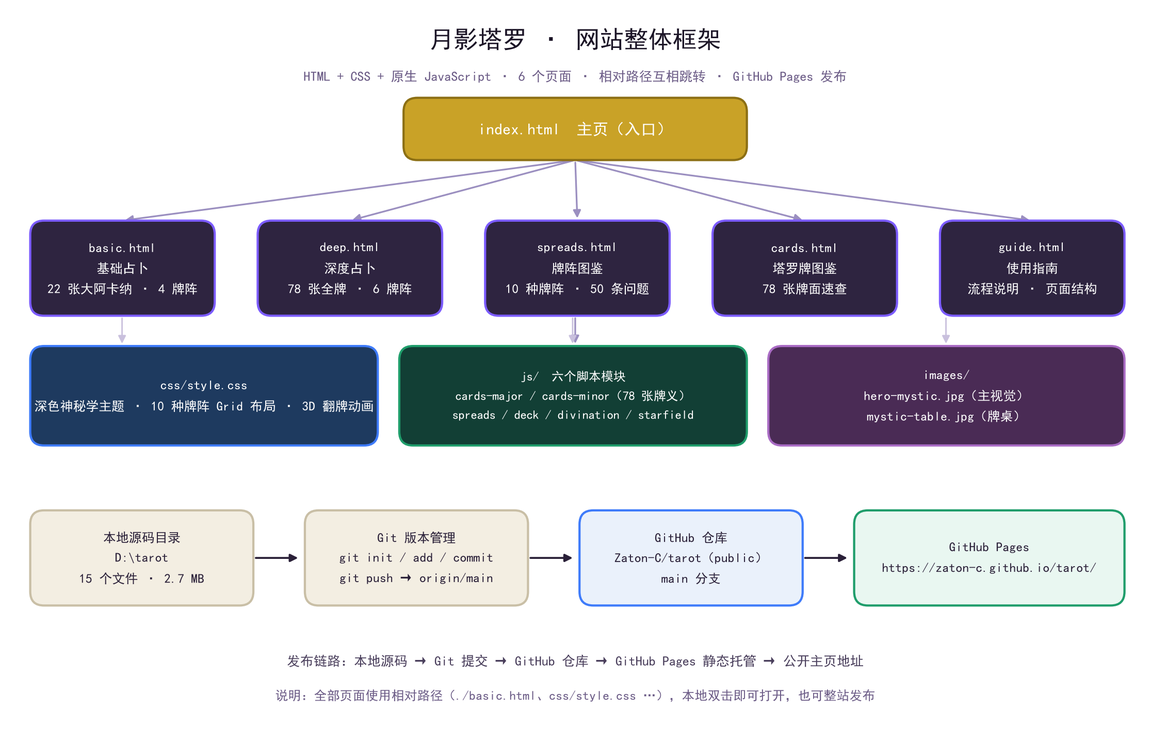
\includegraphics[width=0.92\textwidth]{images/fig-framework.png}
		\caption{月影塔罗网站整体框架图}
		\label{fig:framework}
	\end{center}
\end{figure}

\subsection{目录结构与文件分工}

网站源文件全部位于同一个目录之下，目录结构如下。其中所有资源引用均为相对路径，因此整份目录可以任意移动、拷贝或整体发布。

\begin{verbatim}
tarot/
|-- index.html          主页（站点入口与总览）
|-- basic.html          基础占卜（22 张大阿卡纳 · 4 种牌阵）
|-- deep.html           深度占卜（完整 78 张 · 6 种牌阵）
|-- spreads.html        牌阵图鉴（10 种牌阵 + 50 条备选问题）
|-- cards.html          塔罗牌图鉴（78 张牌面速查）
|-- guide.html          使用指南（流程说明与页面结构）
|-- css/
|   `-- style.css       全站主题样式（约 30 KB）
|-- js/
|   |-- cards-major.js  22 张大阿卡纳牌义
|   |-- cards-minor.js  56 张小阿卡纳牌义
|   |-- spreads.js      10 种牌阵定义与备选问题
|   |-- deck.js         洗牌、发牌与 SVG 卡面绘制
|   |-- divination.js   四步占卜流程与解读生成
|   `-- starfield.js    星空背景绘制
`-- images/
    |-- hero-mystic.jpg 主视觉插画
    `-- mystic-table.jpg 牌桌插画
\end{verbatim}

\subsection{页面清单}

六个页面的分工如表\ref{tab:pages}所示。除主页外的五个页面既可以从主页的导航栏进入，也可以在各页面顶部的导航栏中互相切换，
任意两个页面之间都可以通过相对路径互相到达。

\begin{table}[htb]
	\centering
	\caption{网站页面清单}
	\label{tab:pages}
	\begin{tabularx}{\textwidth}{l l X l}
		\toprule
		页面文件 & 页面名称 & 主要内容与作用 & 包含牌阵 \\
		\midrule
		index.html & 主页 & 站点总览、主视觉、两条占卜路线入口、功能导航与页脚 & --- \\
		basic.html & 基础占卜 & 四步向导：选牌阵、选问题、洗牌翻牌、生成解读 & 4 种 \\
		deep.html & 深度占卜 & 与基础占卜同流程，但启用完整 78 张牌与更深牌阵 & 6 种 \\
		spreads.html & 牌阵图鉴 & 10 种牌阵的图形示意、适用场景与备选问题库 & 10 种 \\
		cards.html & 塔罗牌图鉴 & 78 张牌的卡面、正逆位牌义、编号与元素速查 & --- \\
		guide.html & 使用指南 & 占卜流程说明、页面结构说明与常见问题解答 & --- \\
		\bottomrule
	\end{tabularx}
\end{table}

\subsection{相对路径与可移植性}

网站中所有页面跳转均写成 \texttt{./basic.html} 形式，样式表与脚本分别写成 \texttt{css/style.css}、
\texttt{js/deck.js} 这样的相对路径，没有任何绝对路径或指向本机的链接。这带来两个直接好处：
一是本地双击 \texttt{index.html} 即可离线浏览全部功能，不必启动任何服务器；
二是把整个目录提交到 GitHub Pages 后，浏览器访问 \url{https://zaton-c.github.io/tarot/} 时，页面之间的跳转与资源加载
和本地完全一致，不需要为线上环境做二次修改。调试过程中我对全站 87 处链接与资源引用做了逐一校验，确认无一处断链。

\section{主页设计}

主页是整个网站的门面，页面效果如图\ref{fig:home}所示。主页自上而下由五个区块组成：顶部导航栏、主视觉横幅、
两条占卜路线对比、特色说明与页脚。

\begin{figure}[htb]
	\begin{center}
		
\includegraphics[width=0.60\textwidth]{images/fig-home.jpg}
		\caption{主页整体效果（截图自 GitHub Pages 线上站点）}
		\label{fig:home}
	\end{center}
\end{figure}

\subsection{视觉基调}

网站通篇采用深色神秘学风格。底色取接近黑的靛紫 \texttt{\#0d0a14}，正文用低饱和的米白，
标题与关键数字用金色 \texttt{\#c9a227} 强调，交互反馈用紫色 \texttt{\#7c5cff}，
形成"夜幕—星辉—烛金"的层次关系。为了让长页面阅读时不沉闷，背景使用 JavaScript 在 canvas 上绘制一层静态星空，
星点位置由程序随机生成并保留少量高光与晕影，视觉上有纵深但几乎不占用 CPU。

\subsection{信息结构}

主页不堆砌功能，而是回答"我该点哪里"这一件事。横幅区用一句口号点明主题，并给出两个并排的主按钮：
左侧「基础占卜 · 22 张大阿卡纳」，右侧「深度占卜 · 完整 78 张」，把用户按需求分流；
其下的「两条占卜之路」卡片区进一步解释两种占卜的适用场景差异——基础占卜快、直接、不纠缠细节，
深度占卜看得到时间线、阻力与可执行的步骤。顶部导航栏固定包含主页、基础占卜、深度占卜、牌阵图鉴、塔罗牌图鉴与使用指南六个链接，
页脚再次给出这六个入口并标注课程设计信息，保证用户在任意长页面滚动后都能一键回到其它页面。

\section{分页面设计}

\subsection{基础占卜页（basic.html）}

基础占卜页是四步向导式交互，页面自上而下用编号圆点标出"选择牌阵 $\rightarrow$ 选择问题 $\rightarrow$ 洗牌抽牌 $\rightarrow$ 阅读解读"四个步骤，
当前步骤高亮并可点击回跳。步骤一列出本级别的 4 种牌阵，每种牌阵用 CSS Grid 画出迷你牌型缩略图并标明张数，如图\ref{fig:basic-spread}所示。

\begin{figure}[htb]
	\begin{center}
		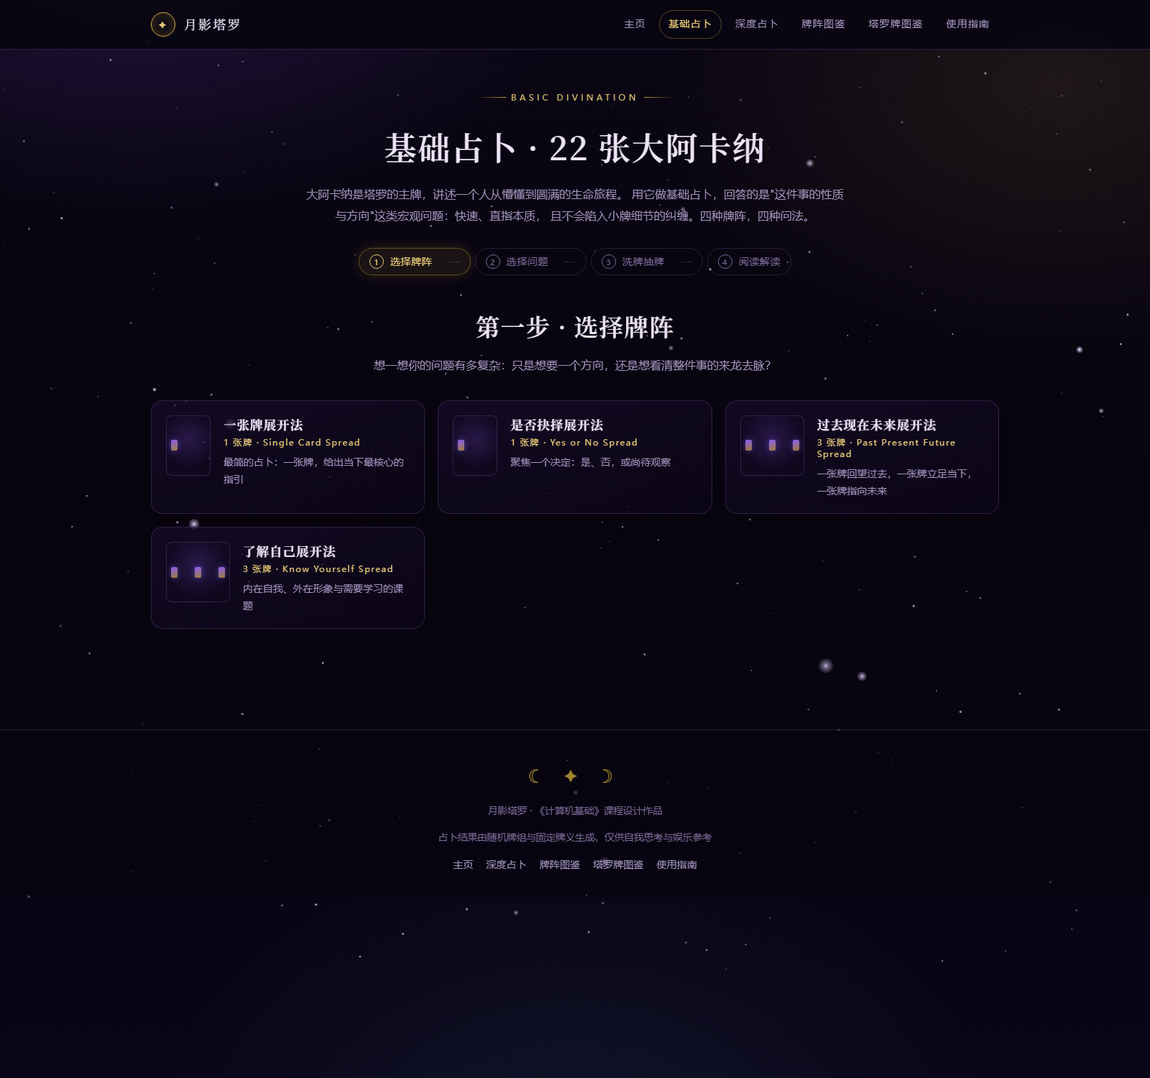
\includegraphics[width=0.58\textwidth]{images/fig-basic-spread.jpg}
		\caption{基础占卜：第一步选择牌阵}
		\label{fig:basic-spread}
	\end{center}
\end{figure}

步骤二给出该牌阵对应的 5 条备选问题（也可以自己输入不超过 60 字的自定义问题）。步骤三是本站的核心交互：
点击「开始洗牌」后牌堆做洗牌动效，随后按牌阵布局把牌发到桌面上，用户必须亲手逐张点击翻牌，
每翻一张计数器就更新一次，全部翻开后「揭示我的解读」按钮才会点亮——这种"必须动手"的节奏让占卜有了仪式感。
图\ref{fig:basic-board}是基础占卜"过去现在未来展开法"翻牌后的实拍效果。

\begin{figure}[htb]
	\begin{center}
		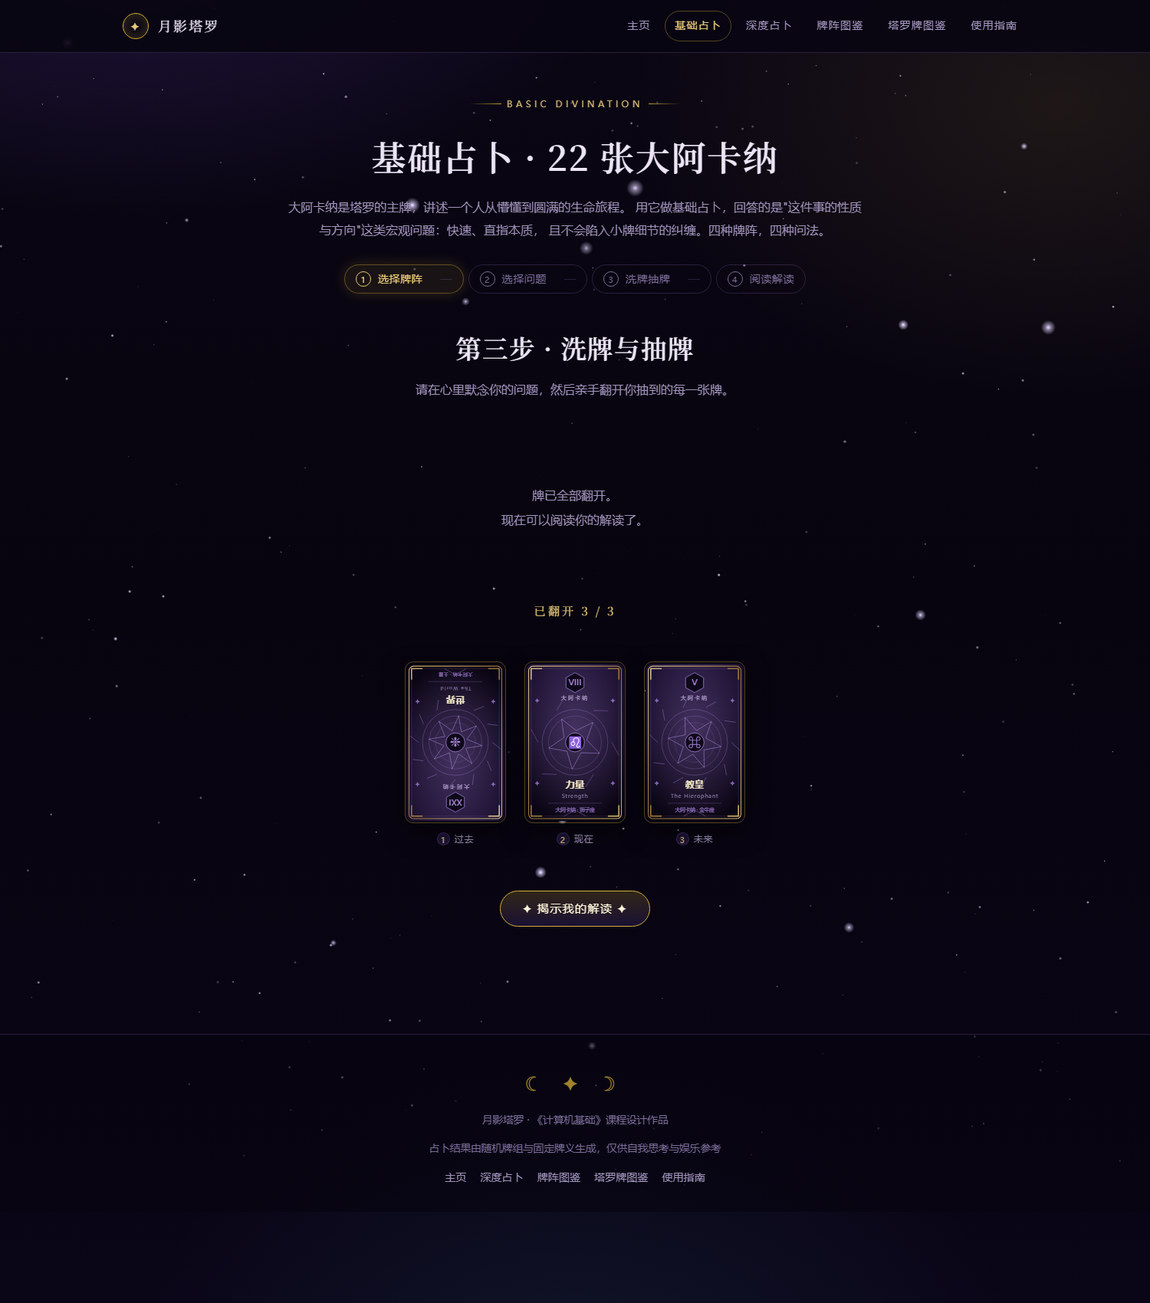
\includegraphics[width=0.50\textwidth]{images/fig-basic-board.jpg}
		\caption{基础占卜：三张牌展开并全部翻开}
		\label{fig:basic-board}
	\end{center}
\end{figure}

步骤四由程序生成解读，内容分四块：逐张牌义（牌名、正逆位、所属花色/元素、牌义与建议）、
元素能量分析（火、水、风、土四种元素在本次抽牌中的占比及解读）、综合结论（结合首尾两张牌给出整体倾向）
以及三条可执行的行动建议。对「是否抉择」这一特殊牌阵，系统还会额外给出"做"与"不做"的倾向判断。
图\ref{fig:basic-result}是一次完整解读的界面。

\begin{figure}[htb]
	\begin{center}
		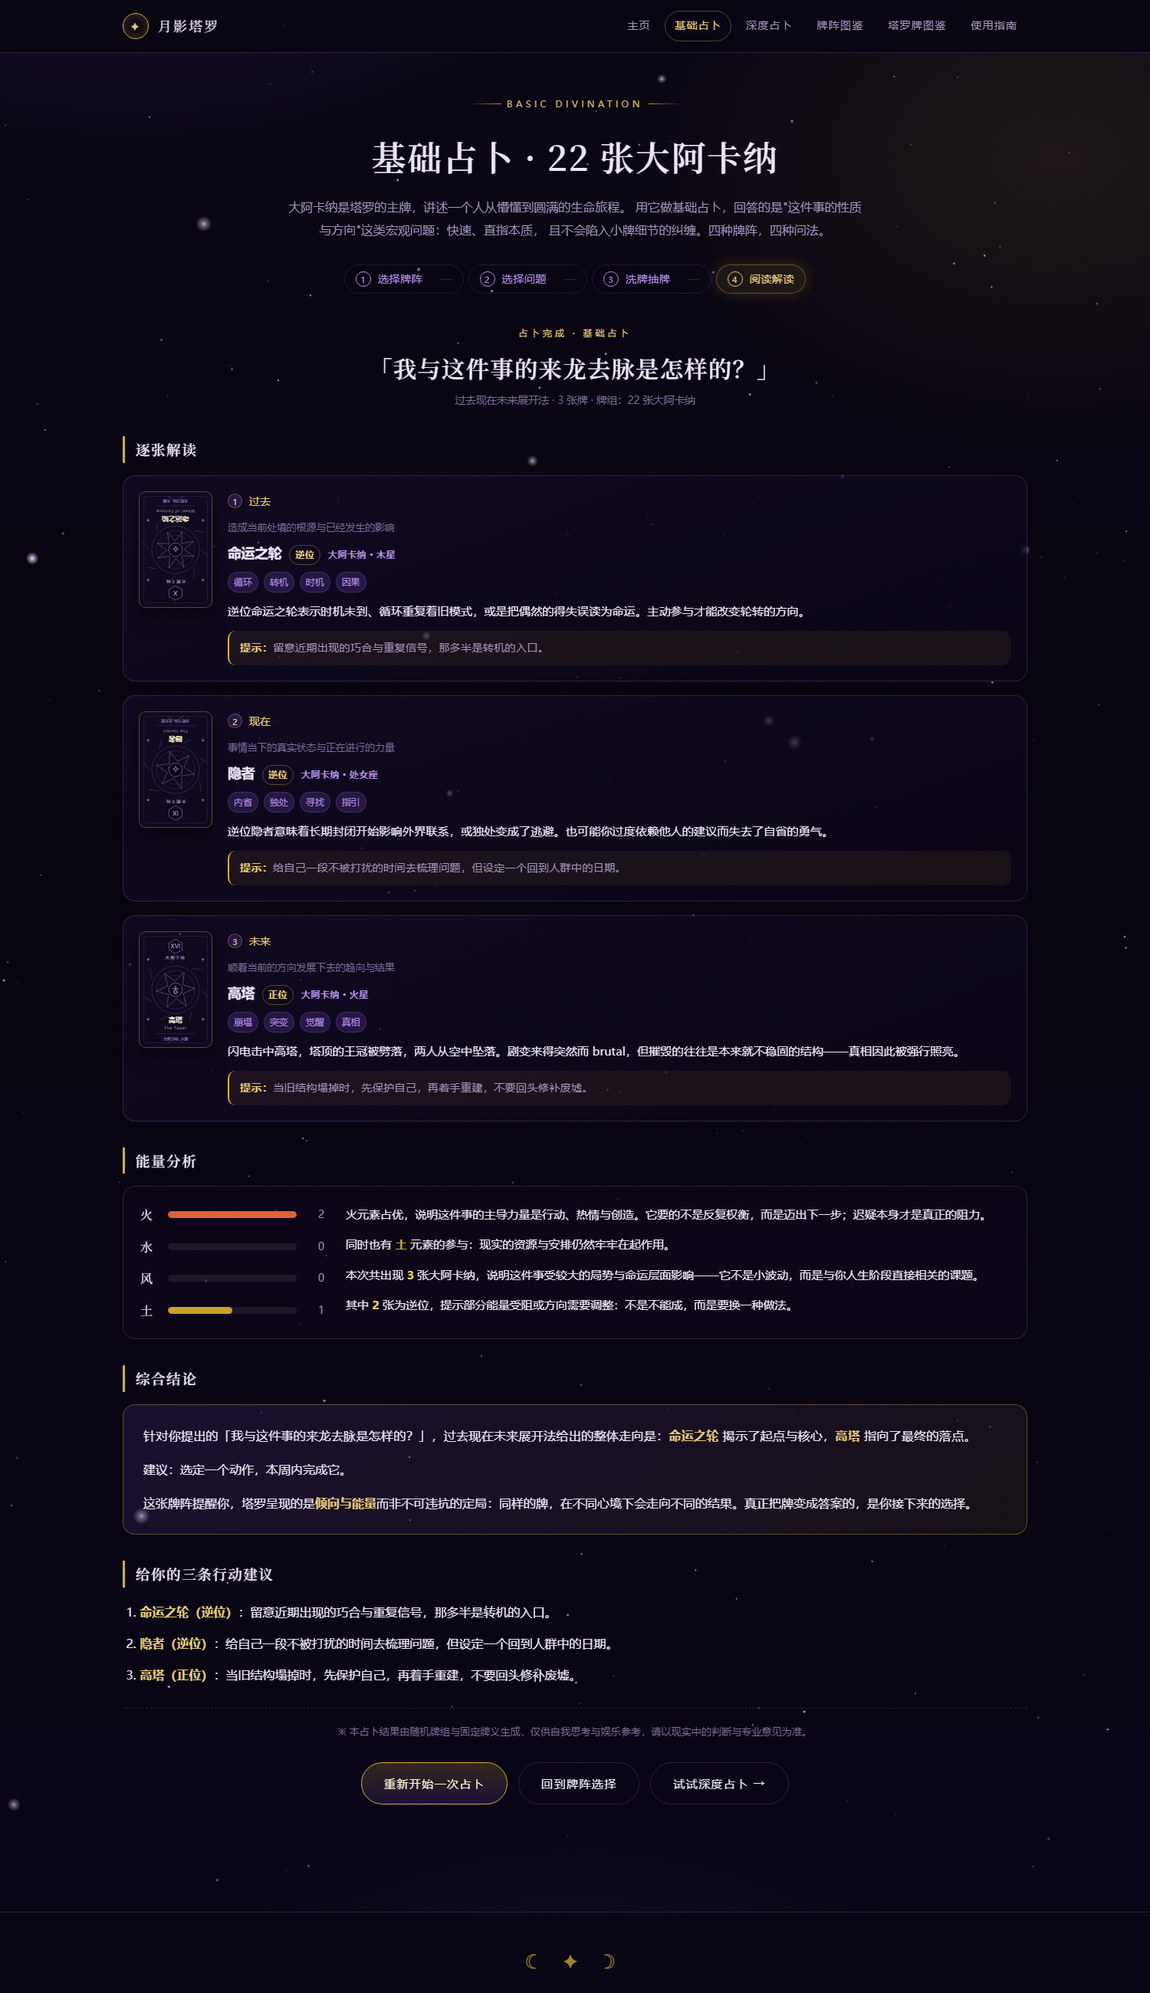
\includegraphics[width=0.44\textwidth]{images/fig-basic-result.jpg}
		\caption{基础占卜：自动生成的解读报告}
		\label{fig:basic-result}
	\end{center}
\end{figure}

\subsection{深度占卜页（deep.html）}

深度占卜页与基础占卜共用同一套向导与解读引擎，区别在于牌库从 22 张大阿卡纳扩展为完整 78 张，
牌阵也从 4 种扩展到 6 种（5 张到 10 张不等），牌阵布局涵盖横向三列、五芒星、菱形等更为复杂的形态。
图\ref{fig:deep-board}是「元素五芒星展开法」的展开效果，可以清楚看到土、火、水、风四种元素被分别安排在五个位置上。

\begin{figure}[htb]
	\begin{center}
		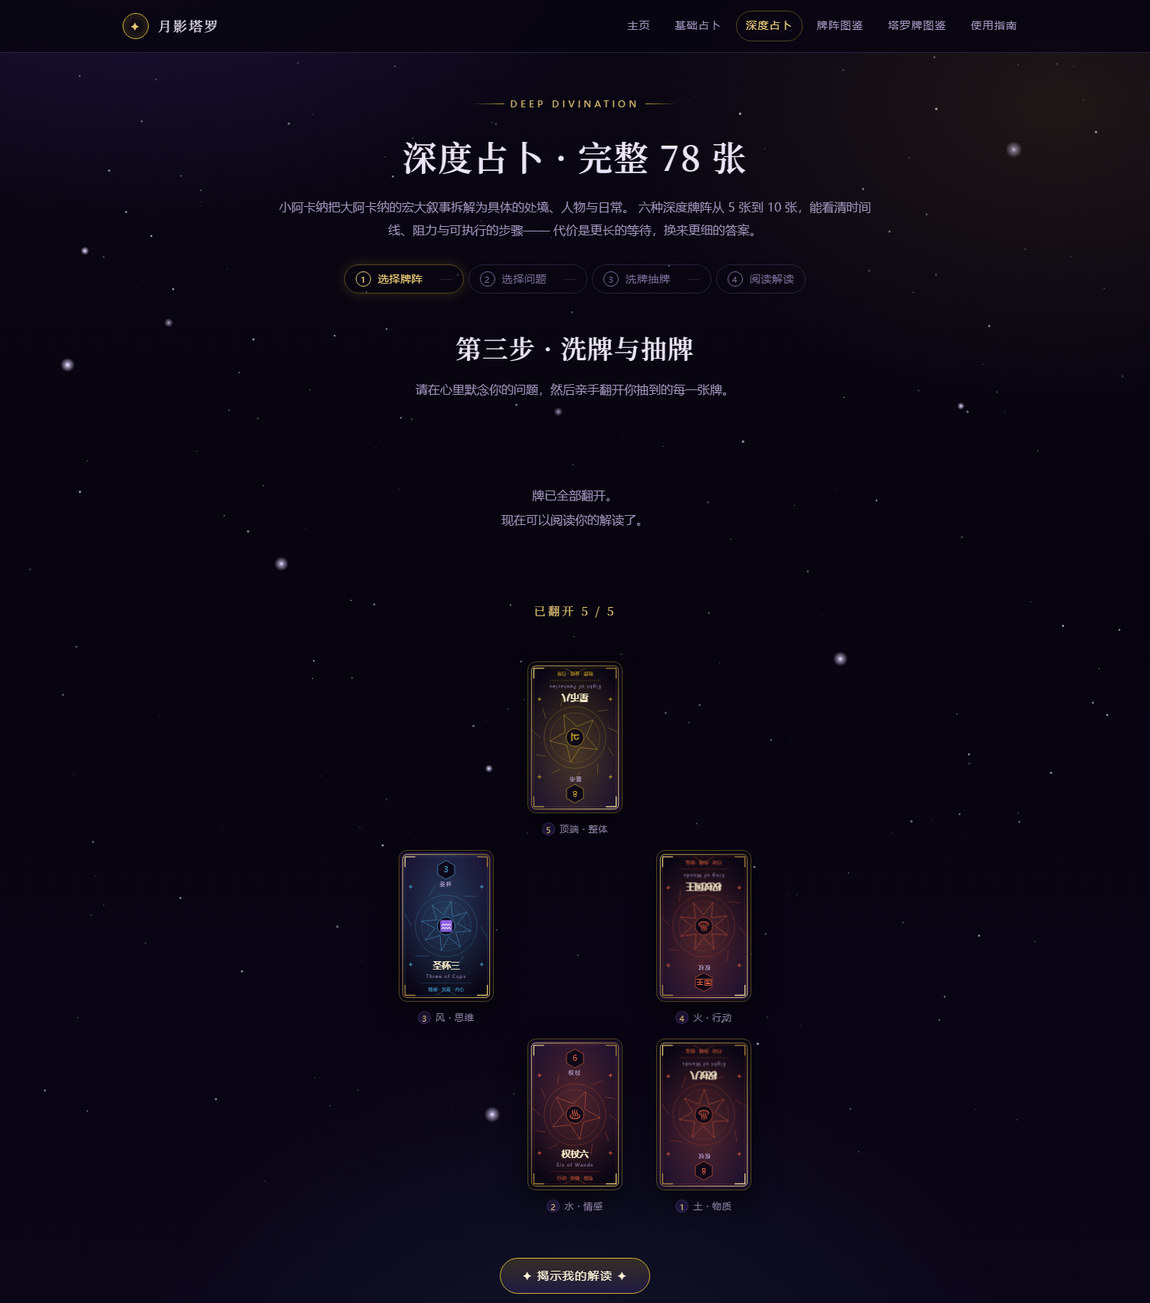
\includegraphics[width=0.50\textwidth]{images/fig-deep-board.jpg}
		\caption{深度占卜：元素五芒星牌阵展开}
		\label{fig:deep-board}
	\end{center}
\end{figure}

当牌阵为 5 张或 10 张时，解读页还会给出更完整的能量结构分析，元素占比条形图不再稀疏。
图\ref{fig:deep-result}是一次深度占卜的解读界面，与基础占卜相比，单次解读的文字量明显更大。

\begin{figure}[htb]
	\begin{center}
		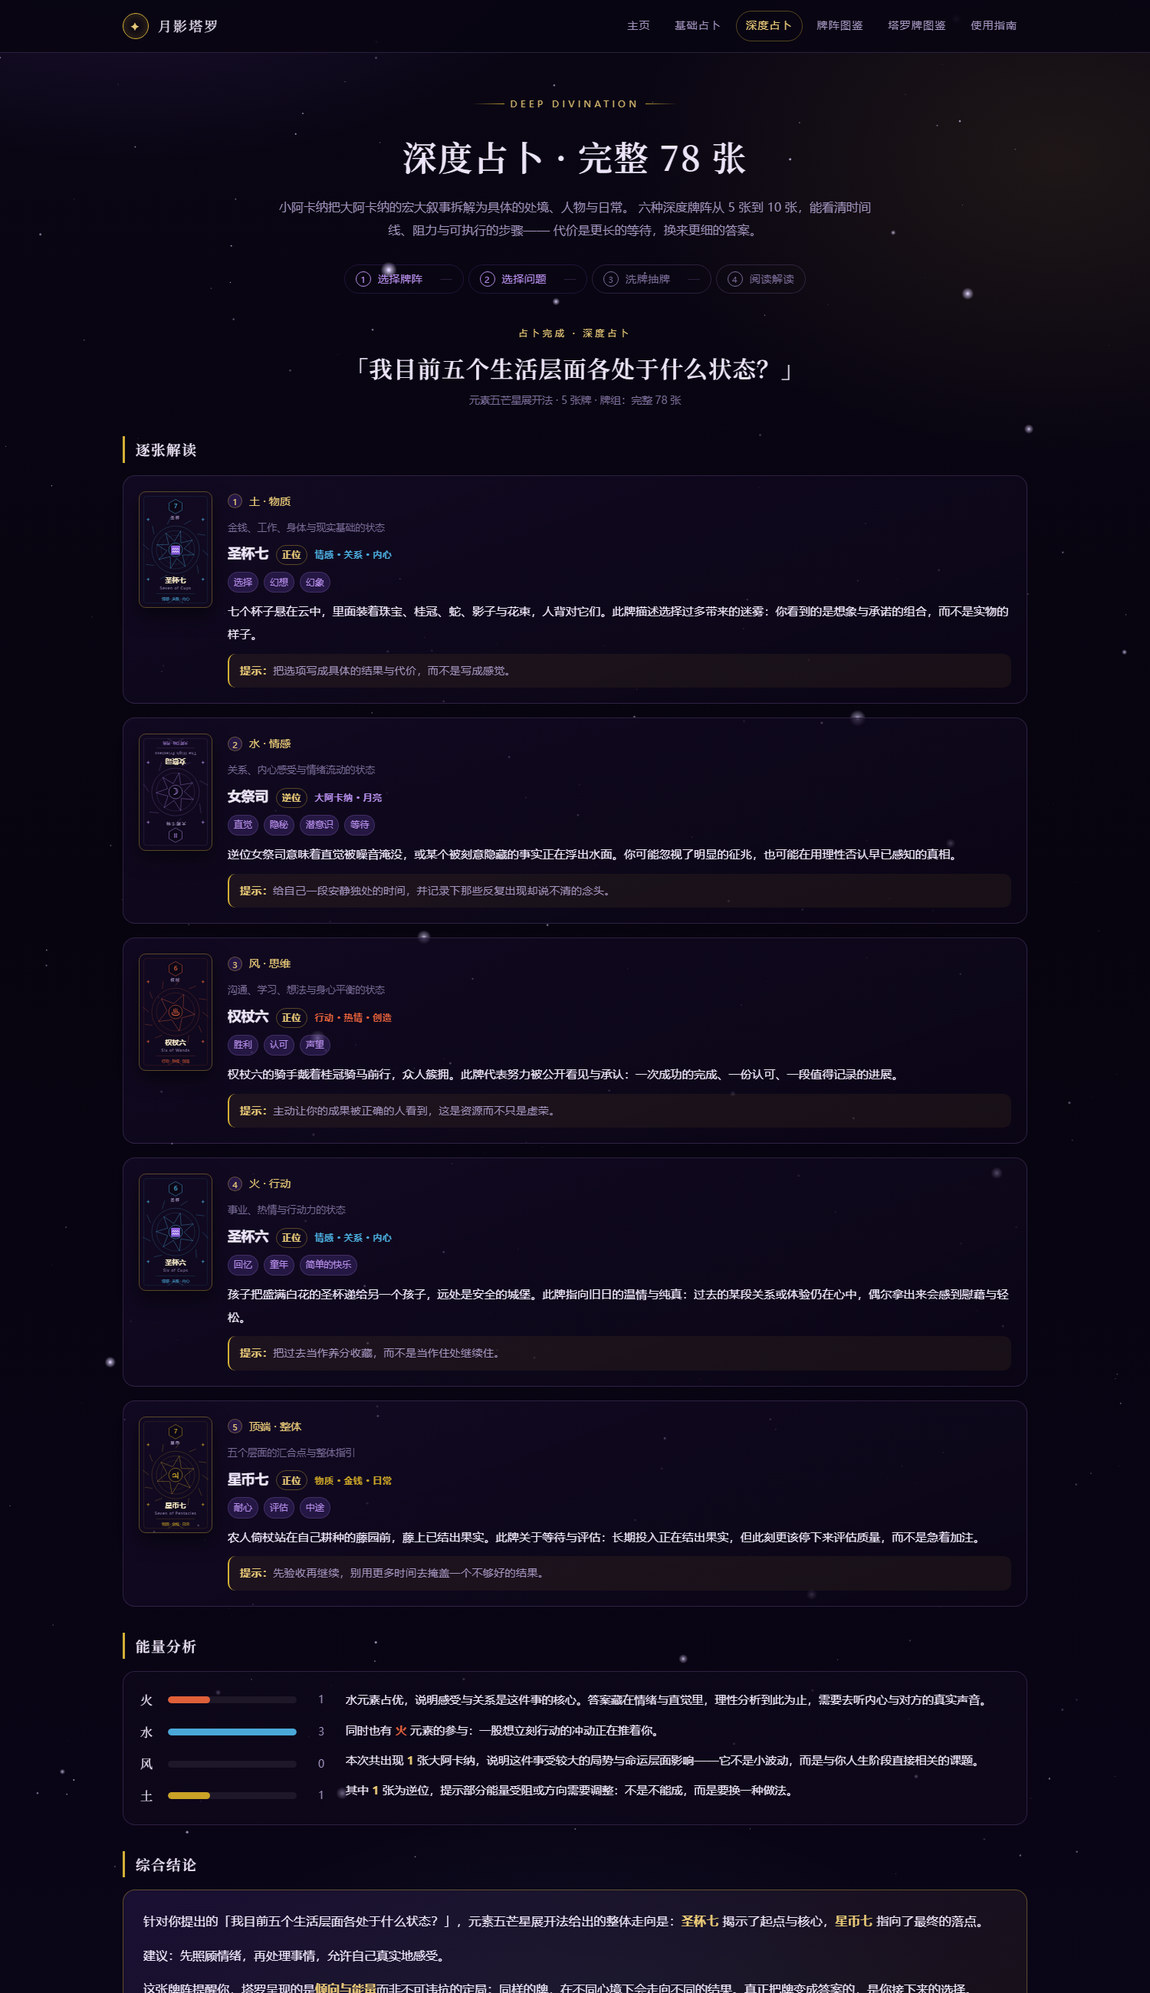
\includegraphics[width=0.44\textwidth]{images/fig-deep-result.jpg}
		\caption{深度占卜：五张牌的完整解读}
		\label{fig:deep-result}
	\end{center}
\end{figure}

\subsection{牌阵图鉴页（spreads.html）}

牌阵图鉴页把 10 种牌阵一次性摊开供用户挑选，如图\ref{fig:spreads}所示。
每种牌阵都用与实际占卜时一致的牌型示意图形呈现，并标注张数、英文名、一句话适用场景和该牌阵下的备选问题数量，
共提供 50 条备选问题。这一页相当于一张"占卜说明书"，让用户在正式抽牌前先想清楚要问什么、要用几张牌。

\begin{figure}[htb]
	\begin{center}
		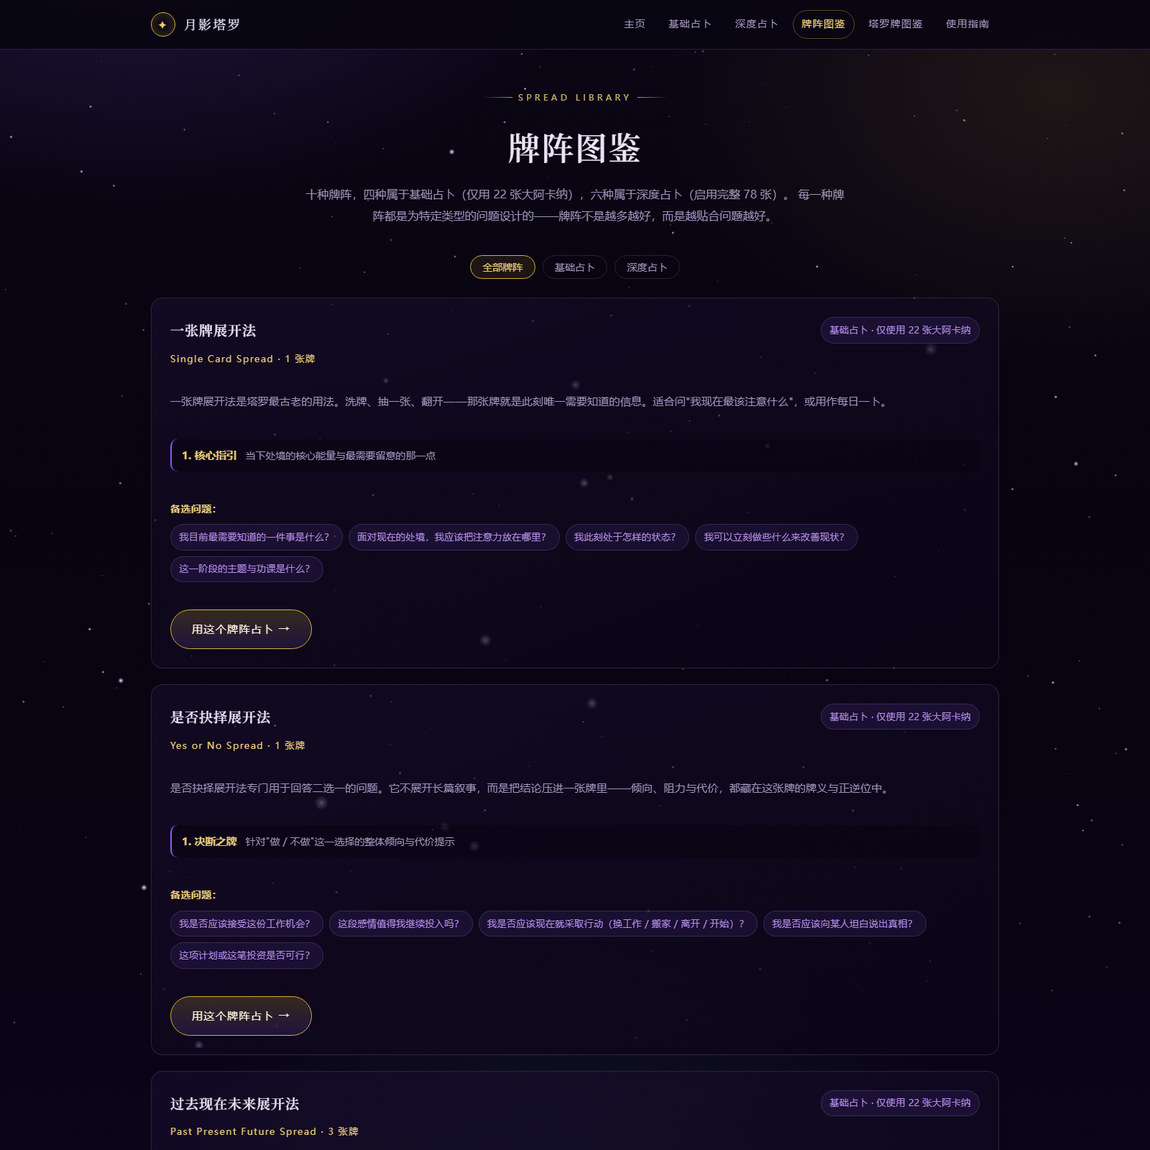
\includegraphics[width=0.58\textwidth]{images/fig-spreads.jpg}
		\caption{牌阵图鉴页}
		\label{fig:spreads}
	\end{center}
\end{figure}

\subsection{塔罗牌图鉴页（cards.html）}

塔罗牌图鉴页提供完整 78 张牌的速查，如图\ref{fig:cards}所示。每张牌都以卡片形式排布，
点击可展开正面牌义、逆位牌义与行动建议。页面上方提供按大阿卡纳、小阿卡纳以及四花色的筛选，
并按火、水、风、土四种元素标注，便于在做深度解读时快速回查某一张牌的来历。

\begin{figure}[htb]
	\begin{center}
		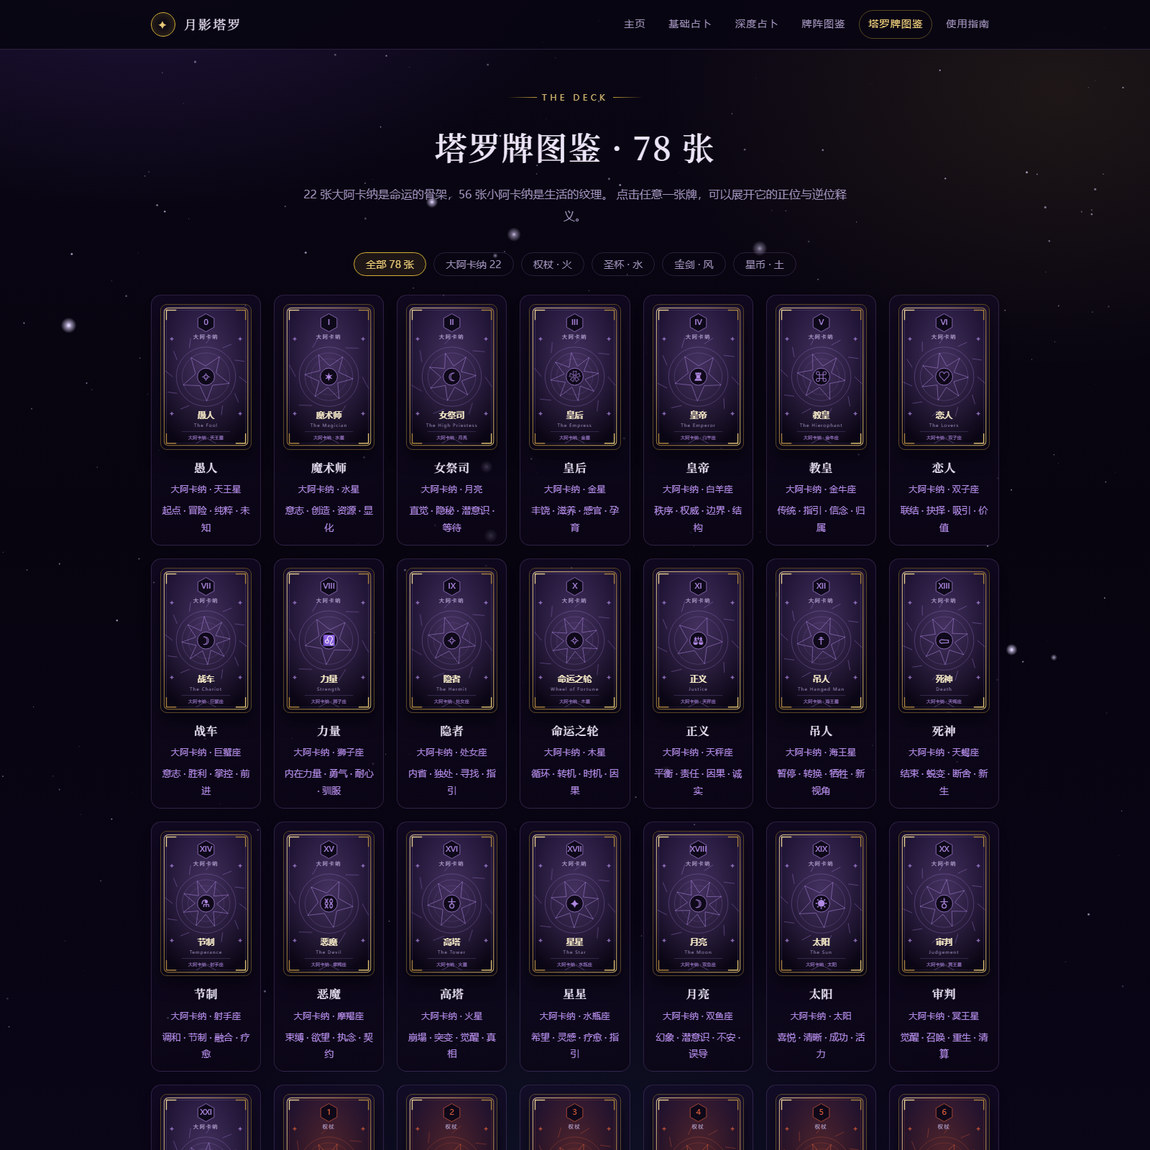
\includegraphics[width=0.58\textwidth]{images/fig-cards.jpg}
		\caption{塔罗牌图鉴页（78 张牌）}
		\label{fig:cards}
	\end{center}
\end{figure}

\subsection{使用指南页（guide.html）}

使用指南页是面向新用户的说明文档，包含占卜四步流程图解、两个级别的差异对照、
站点页面结构说明以及常见问题（如逆位是什么意思、正逆位出现的概率、为什么必须亲手翻牌等），
如图\ref{fig:guide}所示。

\begin{figure}[htb]
	\begin{center}
		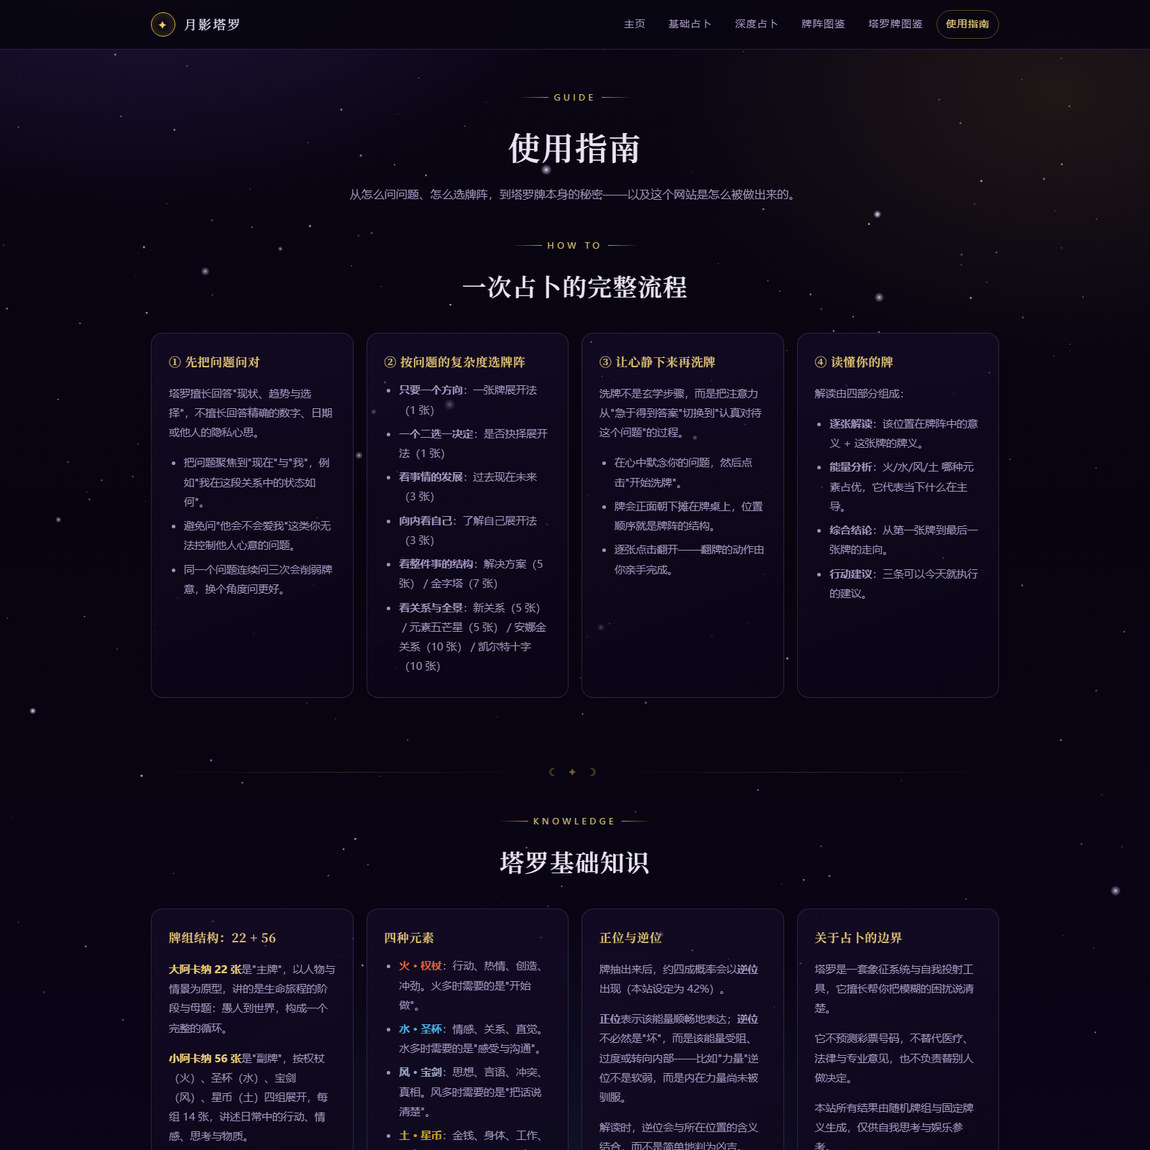
\includegraphics[width=0.58\textwidth]{images/fig-guide.jpg}
		\caption{使用指南页}
		\label{fig:guide}
	\end{center}
\end{figure}

\subsection{版本管理与网页发布}

网站使用 Git 进行版本管理，并在 GitHub Pages 上公开发布，这也是作业中"推送形成主页链接"这一考察项的落实。
本地源目录为 \texttt{D:/tarot}，在该目录中依次执行 \texttt{git init -b main}、
\texttt{git add .}、\texttt{git commit}、\texttt{git push -u origin main}，
首次推送生成提交 \texttt{6dd5496}（15 个文件，3220 行新增），提交记录如图\ref{fig:ghcommits}所示。

\begin{figure}[htb]
	\begin{center}
		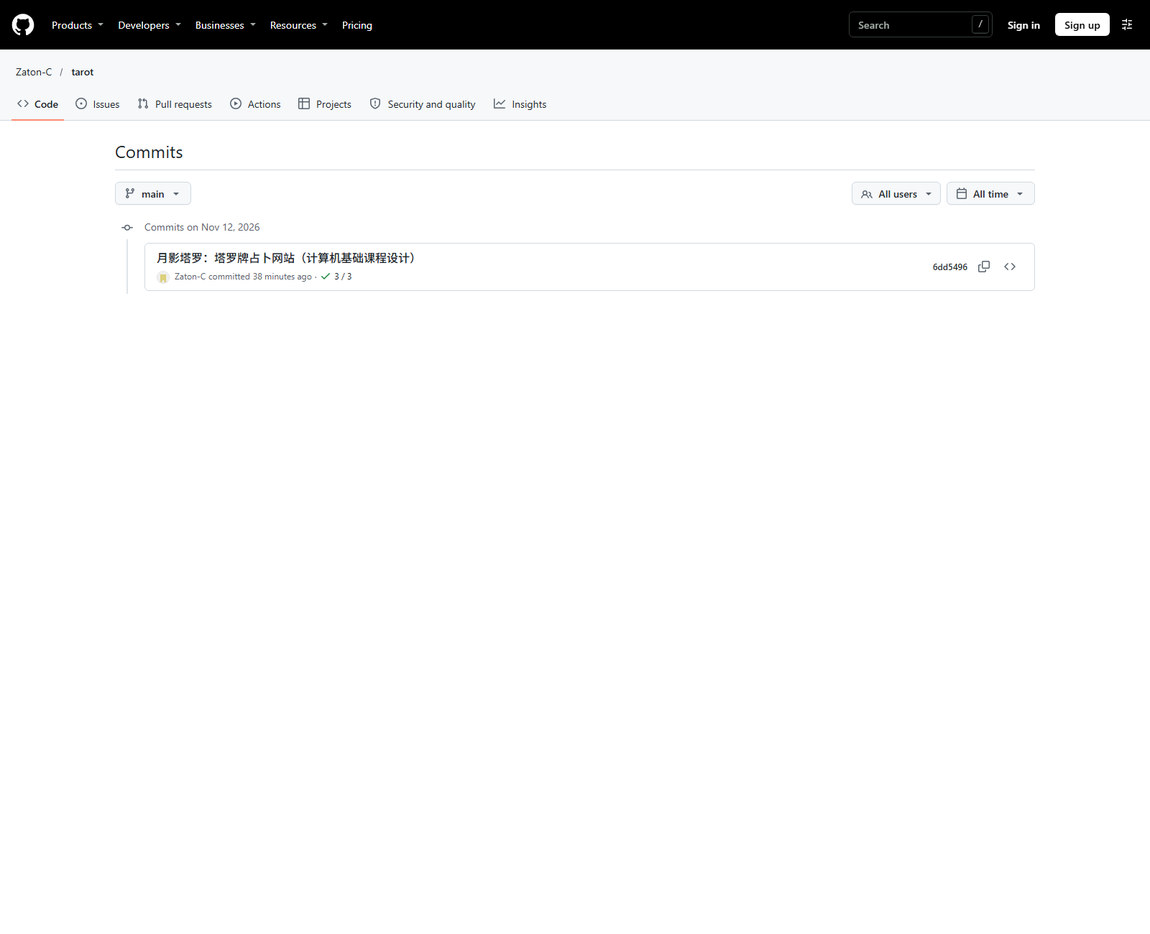
\includegraphics[width=0.95\textwidth]{images/fig-github-commits.jpg}
		\caption{GitHub 仓库提交记录（考察项 8 的过程证据）}
		\label{fig:ghcommits}
	\end{center}
\end{figure}

随后在仓库的 Settings 中将 Pages 的发布来源设置为 \texttt{main} 分支根目录，
GitHub 自动完成构建，构建状态为 \texttt{built}，最终得到公开主页地址
\url{https://zaton-c.github.io/tarot/}。仓库主页如图\ref{fig:ghrepo}所示，
地址栏显示站点已成功上线，右侧同时给出该仓库的 Pages 访问链接。

\begin{figure}[htb]
	\begin{center}
		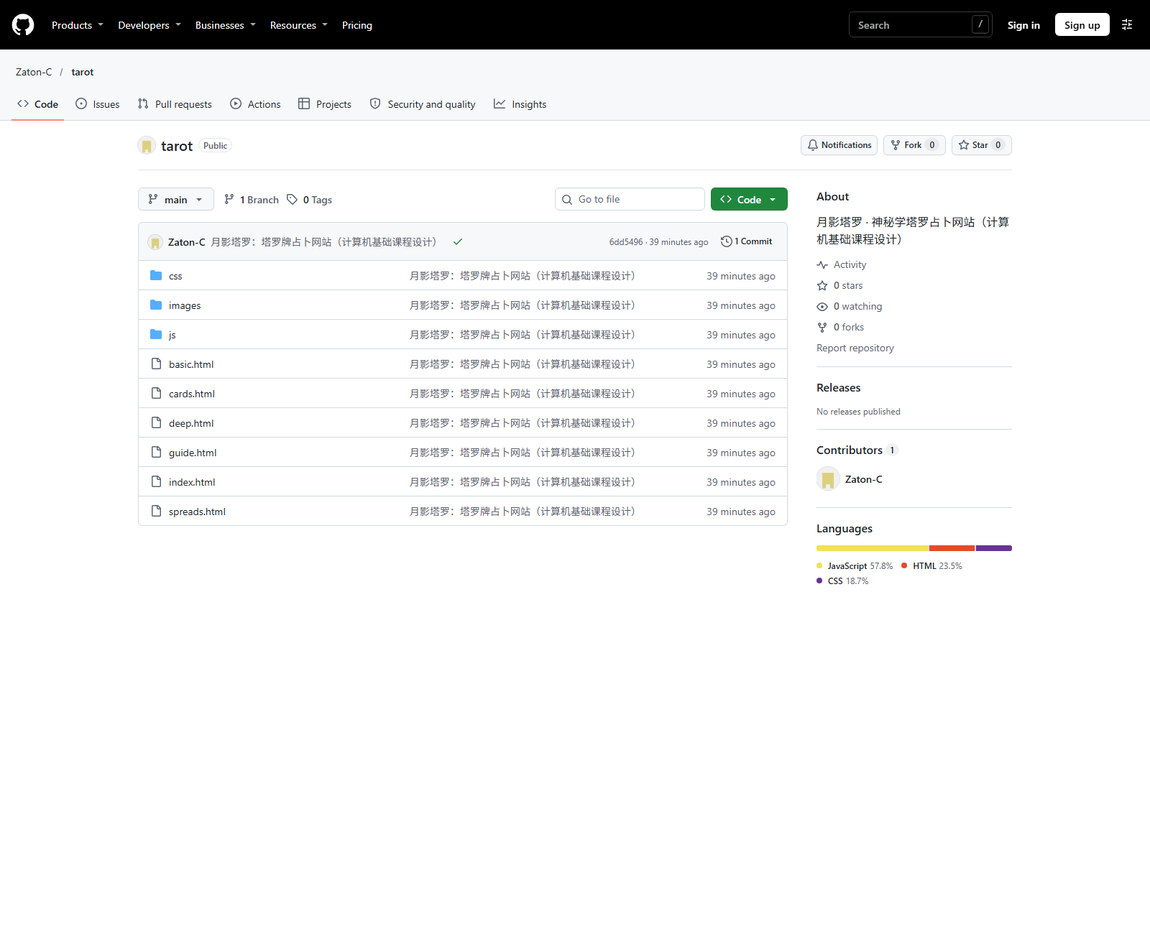
\includegraphics[width=0.88\textwidth]{images/fig-github-repo.jpg}
		\caption{GitHub 仓库主页与 Pages 发布状态}
		\label{fig:ghrepo}
	\end{center}
\end{figure}

\section{网页设计小结}

\subsection{设计与实现中遇到的问题}

网站从初版到定稿共修复了若干真实问题，汇总如表\ref{tab:bugs}所示。

\begin{table}[htb]
	\centering
	\caption{开发调试中遇到的主要问题与解决办法}
	\label{tab:bugs}
	\begin{tabularx}{\textwidth}{l l X}
		\toprule
		问题现象 & 原因分析 & 解决办法 \\
		\midrule
		卡面显示 \texttt{undefined} & 牌义数据缺少 \texttt{type} 字段，渲染时取到空值 & 为 78 张牌补齐 \texttt{type} 等字段 \\
		元素能量统计恒为 0 & \texttt{cardElement()} 返回的是"灵 $\cdot$ 风"这类复合值，无法参与元素计数 & 改为返回纯元素，统计恢复正常 \\
		长页面无法滚动到底 & \texttt{body} 上的 \texttt{overflow-x:hidden} 使 body 成为滚动容器 & 把该属性移到 \texttt{html} 上 \\
		部分机器上星空背景显示异常 & 全屏 canvas 每帧重绘，帧率与 GPU 状态影响合成 & 改为一次性静态绘制，只画一帧 \\
		步骤面板文字半透明 & 入场动画的 \texttt{animation-fill-mode:both} 保留了动画初始帧的透明度 & 移除该属性，动画只做位移 \\
		推送时无法完成授权 & 环境的登录端点被网络策略阻断，设备码授权无法走通 & 改用系统中已保存的凭据配合 GitHub API 完成建仓与推送 \\
		接口返回 400 解析错误 & PowerShell 默认按本地编码发送 JSON，中文字段导致报文非法 & 统一以 UTF-8 字节序列构造请求体 \\
		\bottomrule
	\end{tabularx}
\end{table}

其中值得一提的是最后两个问题，它们都不是网页本身的问题，而是"如何把作品交出去"的问题。
最初的设想是用 GitHub 的设备码登录完成推送，但当前网络环境下登录端点不可达；
改为读取系统中已保存的 GitHub 凭据、直接调用 GitHub API 建仓并推送后，流程一次贯通。
这让我意识到，版本管理与代码托管平台的使用经验，和前端技术本身同样重要。

\subsection{质量控制与自测}

为了避免"看起来能跑但到处是错"，我在定稿前写了两个自检脚本：一是自动驱动占卜全流程的功能自检页，
逐项检查选牌阵、选问题、洗牌发牌、翻牌计数、解读生成、能量统计、行动建议等行为，基础占卜 34 项、
深度占卜 10 项全部通过；二是全站链接与资源引用的静态扫描，87 处引用零断链。
两个自检脚本在交付前已删除，不进入仓库。

\subsection{原创性与合规性}

作业明确要求不得抄袭或直接搬用网上的现成页面。为此，78 张塔罗牌的牌面全部由程序生成：
程序读取牌号做哈希运算，据此确定纹章的对称性、元素配色、星辰数量与装饰图案，再用 SVG 画出卡面，
因此每张牌都独一无二，且不涉及任何第三方图片素材的版权问题。全站仅有两张位图插画，
即主页的主视觉与牌桌插画，由 AI 辅助生成后手工调整。所有文字内容（78 张牌义、10 种牌阵说明、50 条备选问题、
解读文案与行动建议）也均为本次自行撰写。

\subsection{性能与使用体验}

由于没有引入任何框架与外部资源，网站的静态资源总量很小：单个页面的 HTML 约 4--11 KB，
脚本合计约 80 KB，样式表约 30 KB，整站在 GitHub Pages 上打开速度很快。
程序化 SVG 卡面避免了 78 张图片的加载开销，翻牌动画由 CSS 3D transform 实现，交互流畅。

\section{课程的收获和建议}

\subsection{计算机基础知识}

通过本专题，我第一次比较完整地走完了"设计 $\rightarrow$ 编码 $\rightarrow$ 调试 $\rightarrow$ 部署"这一条链路。
最大的收获是意识到网页并不是"若干个 HTML 文件的堆叠"，而是一个有结构的系统：页面之间要用相对路径彼此可达，
样式与脚本要分层管理，资源命名要统一，交互状态要有清晰的生命周期。
建议在讲授时可以补充一个"完整的小项目"示例，把目录组织、代码复用、调试技巧和发布流程串起来演示，
比分散讲解单个知识点更容易建立整体认识。

\subsection{文档撰写工具LaTeX}

本专题让我第一次接触到 LaTeX，并用课程提供的实验报告模板完成了这份报告。
它的价值在于"内容与排版分离"的思路：写内容的人不必关心版式，而版式由模板统一保证，
这与前端开发中"结构、表现、行为分离"的思想是相通的。
本报告即采用课程模板编译生成，目录、页眉页脚、标题编号与参考文献样式均由模板自动完成。
建议在课上多演示模板的样式定义文件如何工作，并说明常见宏包缺失时该如何排查，
这样初学者遇到编译错误时能更快定位问题。

\subsection{编程工具Python}

Python 在本课程设计中主要承担了三类工作：一是批量处理牌义与牌阵的静态数据，
二是生成自检脚本，驱动浏览器完成全流程的自动化检查，三是绘制报告中的框架图与批量生成插图。
我体会到 Python 最大的价值在于"把重复劳动交给脚本"，
面对 78 张牌这种规模的数据，人工检查几乎不可能，而脚本几秒钟就能跑完并逐条列出结果。
建议增加一次"用脚本处理真实数据"的演示，哪怕数据量不大，也能让同学直观感受到自动化的意义。

\subsection{图像设计软件Photoshop}

主视觉与牌桌两张插画的配色方案，主要是在 Photoshop 中反复调整出来的：先定好主色与辅色的明度关系，
再压暗整体饱和度，让插画能和网页的深色背景自然融合而不抢文字的视觉焦点。
通过这次实践，我理解了"配图不是贴上去就行"——图片的色调、亮度和留白必须与页面整体设计配合，
否则再好的素材也会破坏页面的一致性。建议在讲评作业时，多展示一些"配图前后对比"的实例，
说明主观审美背后的可操作规则。

\subsection{版本管理软件Git}

Git 是本次设计中收益最大的工具。从最初的 \texttt{git init}、\texttt{commit}，
到 \texttt{clone} 出工作副本、把课程工作目录和源码目录分开管理，再到解决推送授权问题，
让我真正理解了版本管理的意义：它记录的是"过程"，而不只是"结果"。
课程提供的 Readme 中提到用 \texttt{git revert} 与 \texttt{reset} 回退版本，我也在本地实验了二者的区别——
前者生成一次新提交来抵消旧改动、保留历史，后者直接移动分支指针、丢弃提交。
建议在教学中多用真实的错误提交来演示回退，比抽象讲解命令更有说服力。

\subsection{网页制作Dreamweaver}

课程以 Dreamweaver 讲解网页制作，而我实际开发时基本是手写代码加浏览器开发者工具调试。
这让我体会到工具只是载体：模板、代码提示、实时预览确实能提高起步速度，但真正决定效率的，
是对 HTML 结构、CSS 盒模型与选择器优先级的理解。建议课程保留可视化工具的演示，
同时补充"代码视图 + 开发者工具"的对照演示，帮助同学在工具之外也能独立定位问题。

\clearpage

\nocite{*} %% 作用是不对文献进行引用，但可以生成文献列表

%本模板使用 \nocite{*} 生成文献列表，如需正式引用可取消下面两行注释并运行 bibtex
%\bibliographystyle{Experimental_Report}
%\bibliography{Experimental_Report}

\end{document}
